\documentclass{fithesis}

\usepackage{lmodern}
\usepackage[czech]{babel}
\usepackage[utf8]{inputenc}
\usepackage{cmap}
\usepackage{graphicx}
\usepackage[T1]{fontenc} %formátuje české znaky - důležité
\usepackage[plainpages=false, pdfpagelabels]{hyperref}
\usepackage{hyperref}
%\usepackage{makeidx}
%\makeindex

%\bibliographystyle{unsrt}


%\makeindex
\thesistitle{Integrace DMS a workflow v Liferay Portal}
\thesissubtitle{Diplomová práce}
\thesisstudent{Marek Tlačbaba}
\thesiswoman{false}
\thesisfaculty{fi}
\thesisyear{2014}
\thesisadvisor{RNDr. Jaroslav Ráček, Ph.D.}


\begin{document}

\FrontMatter
\ThesisTitlePage

\begin{ThesisDeclaration}
Prohlášení\AdvisorName
\end{ThesisDeclaration}

\begin{ThesisThanks}
Poděkování
\end{ThesisThanks}

\begin{ThesisAbstract}
Abstrak
\end{ThesisAbstract}

\begin{ThesisKeyWords}
Klíčová slova
\end{ThesisKeyWords}


\MainMatter
\setcounter{secnumdepth}{4}
\tableofcontents

\chapter{Úvod}
Oficiální zadání

Popsat principy tvorby podnikových portálů. Zaměřit se zejména na otázku implementace workflow pro procesy pracující s vnitropodnikovými dokomenty. Pro Liferay Portal verze CE analyzovat, navrhnout, implementovat, otestovat a zdokumentovat vlastní grafický workflow editor pracující v základní notaci BPMN, který bude plně kompatibilní se standardním workflow systémem, který je součástí Liferay Potral CE. Výstup bude mít podobu funkčního prototypu.

\chapter{Podnikové portály}

Pojem portál bývá definován různými způsoby v závislosti na situaci, ve které je používán. Dříve se portály zaměřovaly hlavně a jenom kolem jednotného přístupu k informacím nezávisle na jejich původu a umístění. S~dalším vývojem informačních technologií se postupně tento přístup dále rozšiřoval a~do definice portálu přibyly pojmy jako integrace a agregace služeb a aplikací. 

V následujícím textu je uvedno několik definic portálu a podnikového portálu.

\begin{itemize}

\item Například Gála definoval portál jako jednotné rohraní, ve kterém lze pracovat s běžnými službami a nástroji jako jsou, například zpravodajství a~komunikace, mimo to je v něm zaručen přístup k všeobecným aplikacím jako jsou vlastní stránky a blogy, a k aplikacím specializovaným, například slovníkům. \cite{gala}

\item Tato definice portálu je převzata ze standardu JSR-286 a zní následovně: Portál je webová aplikace, která (obvykle) poskytuje možnost personalizace, autentifikace, agregace obsahu z různých zdrojů a slouží jako prezentační vrstva informačních systémů. Agregací se rozumí integrace obsahu z různých zdrojů v rámci jedné webové stránky. Portál může mít vysoce propracované nástroje pro personalizaci, které poskytují obsah upravitelný podle přání uživatele. Stránky portálu mohou mít různé skupiny portletů \footnote[1]{Bližší informace v dalších částech této práce.}, které vytvářejí obsah pro různé uživatele.  \cite{jsr-286}

\item Předchozí defince se týkají portálu obecně, proto zde uvedu také definici podnikového portálu jako takového. Například podle Čecha je podnikový portál definován jako internetové nebo intranetové stránky, které slouží jako vstupní bod, respektive brána k různým datovým, informačním a znalostním zdrojům v organizaci. Jejich cílem je zpřístupnit tyto zdroje specifické skupině lidí. Může to být jak zákazníkům, tak také vlastním zaměstnacům nebo partnerům. \cite{cech}

\end{itemize}

V předchozích definicích portálu jsou naznačeny některé základní rysy podnikových portálů. Mezi základní vlastnosti můžeme považovat jediný přístupový bod, integrace, federace, přizpůsobivost, personalizace, kontrola přístupu a vyhledávání v podnikovém obsahu, tak jak jsou uvedeny v \cite{enterprise-portal} 

\section{Konkrétní portálová řešení}
Existuje a používá se celá řada konkrétních portálových řešení. Nejčastěji bývají implementovány v jazyce Java a podporují standardy JSR-168 a JSR-286 \footnote[2]{Bližší informace v dalších částech této práce} pro tvorbu portletů v jazyce Java. Existují také portály i pro jiné technologie, například pro platformu .NET je možné využít Microsoft SharePoint, ale nejvíce řešení existuje pro jazyk Java, kde mezi nejznámější patří IBM Websphere Portal, JBoss GateIn, Oracle WebCenter či Liferay Portal. Tyto portály již většinou obsahují velké množství již připravaných portletů, např. wiki, správa souborů, komunikace a další podobné.

V praktické části této práce bude vytvořen portlet pro tvorbu workflow pomocí grafického designeru v portálu Liferay.

\section{Liferay Portal}
Liferay portal je open-source podnikový portál založený na jazyce Java vyvíjený společností Liferay, Inc.. Podporuje specifikace JSR-168 a JSR-286 pro tvorbu portletů v jazyce Java. Liferay Portal je k dispozici ve dvou edicích, Community Edition a Enterprise Edition.

Community Edition je bezplatná verze portálu, která je volně dostupná ke stažení. Tato verze je ale bez oficiální podpory, ta je dostupná pouze prostřednictvím Liferay komunity. Druhá verze portálu, Liferay Portal Enterprise Edition je placená edice. U této verze je kladen velký důraz na stabilitu, bezpečnost a výkon. K této edici patří dlouhodobá podpora od společnosti Liferay, Inc. nebo jejích partenerů.

Ihned po instalaci portálu je k dispozici množství již předinstalovaných portletů. Je možné například ihned využívat wiki, fórům, kalendář, galerii obrázků. Liferay portál podporuje různé způsoby, jak jej lze upravovat či rozšiřovat. Pro změnu vzhledu můžeme využít témata či šablony, dále funkcionalitu portálu je možno rozšířit pomocí portletů, měnit vlastnoti portálu či portletů je umožněno díky tzv. hooks a větší a zásadnější změny přímo v jádru portálu se provádí pomocí pluginu Ext. \cite{developer-guide}

Portál Liferay nabízí svým uživatelům zabezpečené jednotné přihlášení, nástroje pro správu workflow, snadnou instalaci samotného portálu i dalších nových aplikací a rozšíření. Od verze 6.1 CE GA2 umožňuje instalaci rozšíření a aplikací nově také z Liferay Marketplace. Takto je možné stahovat aplikace přímo z rozhraní portálu.

Liferay také obsahuje pokročilý systém pro správu obsahu (Liferay CMS), který umožňuje oprávněným uživatelům vytvářet a správovat obsah webu přímo z prohlížeče a to i bez znalosti programování. S tím také souvisí možnost dělit uživatele do organizací, skupin a uživatelům přidělovat role, podle kterých jim následně zobrazovat různý obsah, aplikace a umožňovat provádět různé akce.

Mezi další vlastnosti portálu patří vícejazyčné uživatelské rozhraní, personalizace portálových stránek, jednoduchá úprava stránek způsobem táhni a pusť, automatické nahrávání souborů.

Liferay také podporuje různé platformy a proto je možné ho provozovat na různých aplikačních serverech, operačních systémech a databázích. Také podporuje různé metody integrace včetně SOAP, REST, RSS a také další proprietární rozhraní.\cite{liferay-features}

To jsou některé z důvodů, proč se podnikový portál Liferay stal rožšířenou a oblíbenou platformou pro vývoj firemních webů a systému v jazyce Java.

\chapter{Vývoj portletů}
V této kapitole bude popsán vývoj portletů, které tvoří obsah portálů.

\section{Portlet}
Portlet je webová aplikace, která poskytuje uživatelům specifický obsah, typicky informaci nebo službu. Portlet je spravován portletovým kontejnerem, který zpracovává požadavky portletu a následně generuje dynamický obsah v podobě fragmentů v některým ze značkovacích jazyků -- HTML, XHTML, WML.  Tyto fragmenty jsou pak spojovány a dohromady vytváří portálovou stránku.

Portletový kontejner má tedy opovědnost za řízení životního cyklu jedntlivých portletů a je v něm také uloženo nastavení uživatele pro daný portlet. Ale jednotlivé části generované jednotlivými portlety slučuje dohromady na stránku portál. Portál a portletový kontejner mohou postaveny jako jedna komponenta ale mohou být také jako komponenty dvě. Na následujícím obrázku 3.1 je zobrazen průběh vytváření stránky v portálu tak, jak bylo již výše naznačeno.

\begin{figure}[htp]
\centering
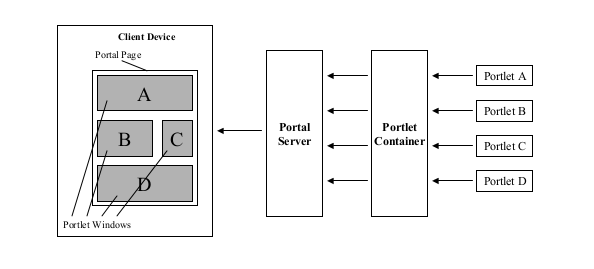
\includegraphics[width=340px]{images/vytvareni_stranky_v_portalu.png}
\caption{Vytváření stránky v portálu (převzato z \cite{jsr-286})}
\end{figure}

\section{Specifikace}
Důvodem pro vytvoření portletové specifikace byla situace, kdy různí dodavatelé používali svá vlastní API, která neumožňovala přenositelnost mezi portálovými servery.

První verze Java Portlet Specification 1.0 (JSR-168) byla vydána v roce 2003. V této specifikaci ještě bylo stále různé nedostatky a chyby, které pak tvůrci portletů stejně řešili každý po svém. To způsobovalo i nadále, že portlety byly mezi portálovými servery stále problematicky přenositelné či nepřenositelné úplně. Proto vznikla druhá verze Java Portlet Specification 2.0 (JSR-286) a ta byla vydána v červnu 2008. Mezi nejdůležitější přínosy patří následující:
\begin{itemize}
\item sdílení parametrů mezi portlety skrz veřejné render parametry,
\item meziportletová komunikace pomocí zasílaní událostí,
\item transformace informací nově definovanými portletovými filtry,
\item možnost portletů poskytovat zdroje jako jsou například PDF soubory.
\end{itemize}
Většina portletových kontejnerů sice poskytuje k základním požadavkům i svá rozšíření. Tyto rozšíření však nemusíme využívat a tak můžeme zachovat myšlenku snadné přenositelnosti.

\subsection{Životní cyklus portletu}
Každý portlet musí implementovat rozhraní \verb|Portlet|. Toto rozhraní obsahuje čtyři základní metody, které musí být implementovány a které řídí životní cyklus portletu - \verb|init(), processAction(), render(), destroy()|.

Metoda \verb|init()| je volána ihned při vytváření portletu a je používána například pro přípravu zdrojů potřebných portletem.

Metoda \verb|processAction()| je volána vždy po provedení nějaké akce uživatelem, když se touto akcí nějak mění stav portletu. Může to být například akce potvrzení formuláře a následné zpracování a uložení dat v databázi.

Metoda \verb|render()| má za úkol generovat fragment stránky, který je pak dostupný uživateli v portletu. V této metodě by se neměl měnit stav portletu.

Poslední metodou je \verb|destroy()|. Ta je volána před odstraněním portletu z paměti. Poskytuje poslední možnost pro uvolnění zdrojů, které byly portletem používány. \cite{jsr-286}

Zpracování požadavků v portletech může procházet několika fázemi zpracování.

\begin{itemize}
\item Render -- vykreslovací fáze, ve které se typicky nemění stav portletu, odpovídá jí metoda \verb|render()|.
\item Action -- portlet zpracovává nějakou akci a typicky mění svůj stav, odpovídá ji metoda \verb|processAction()|.
\item Resource -- portletem je poskytován nějaký zdroj, např. PDF soubory. Aby portlet mohl podporovat tuto funkcionalitu, musí implementovat rozhraní \verb|ResourceServingPortlet|.
\item Event -- portlet přijímá nějakou událost a nějak na ni reaguje. Portlet v tomto případě musí implementovat rozhraní \verb|EventPortlet|.
\end{itemize}

Všechny tyto rozhraní implementuje abstraktní třída \verb|GenericPortlet|. Tato třída obsahuje implementaci všech povinných metoda a několika dalších, které je možné využít.

Po každé action fázi musí následovat fáze render. Pokud se na portálové stránce vyskytuje více portletů, je metoda render zavolána u všech zobrazených portletů. 

\subsection{Režimy portletu}
Portletová specifikace obsahuje tři režimy portletu, které umožňují zobrazit jiný obsah v závislosti na požadovaném úkolu. Tyto režimy využívá metoda \verb|render()|, která podle nich vygeneruje odpovídající obsah.

\begin{itemize}
\item View -- základní režim používaný při klasickém zobrazení portletu na portálové stránce.
\item Edit -- nepovinný, uživateli umožňuje nastavovat portlet.
\item Help -- nepovinný, zobrazuje se nápověda k danému portletu.
\end{itemize}

Ve třídě \verb|GenericPortlet| jsou k těmto účelům definovány metody \verb|doView()|, \verb|doEdit()| a \verb|doHelp()|. Jednotlivé portletové režimy by měli být implementovány přetížením těchto metod. Každý portál si také může definovat vlastní portletové režimy. Každý portlet musí mít zadefinováno, které režimy podporuje.

\subsection{Stavy okna}
Portletová specifikace definuje tři základní stavy.

\begin{itemize}
\item Minimized -- okno portletu je minimalizované.
\item Normal -- původní velikost portletu, které umožňuje zobrazení všech portletů na na portálové stránce.
\item Maximized -- okno portletu skryje ostatní portlety na stránce a zobrazuje se pouze tento maximalizovaný portlet, nebo zakrývá většinu dostupné plochy.
\end{itemize}

\subsection{Struktura poprtálové aplikace}
Portálové aplikace jsou uloženy ve standardní archivním souboru jazyka Java, Web ARchive (WAR). Mohou obsahovat více portletů, servlety, JSP soubory a další. Musí obsahovat webový deskriptor a také navíc portletový deskriptor implementace \verb|portlet.xml|.

\chapter{Workflow}
Jednoznačná definice workflow neexistuje, jelikož každá oblast, ve které je workflow používáno, si ho definuje po svém. Obecně je ale možné definovat workflow jako proces automatizace podnikových procesů. O sjednocení této terminologie se již v roce 1996 pokusila institut Workflow Management Coalition (WfMC), kdy vydal terminologický slovník, ve kterém je workflow definováno takto: 

Workflow zanamená automatizaci celého nebo části podnikového procesu, během kterého jsou dokumenty, informace nebo úkoly předávány od jednoho účastníka procesu k druhému podle sady procedurálních pravidel tak, aby se dosáhlo nebo přispělo k plnění celkových/globálních podnikových cílů. \cite{wfmc}

V počítačových systémech je workflow definováno jako systém řízení workflow. V tomto systému je možné workflow definovat, vytvořit a celý průběh procesu řídit. Mezi jeho úkoly patří provádět definici procesu, komunikovat s účastníky workflow, případně spouštět další aplikace nutné k vykonání workflow.


\section{Typy workflow systému}
Workflow systémy se mohou dělit do několika skupin podle různých hledisek či typů. \cite{workflow}

\subsection{Hledisko charakteru procesů}
\begin{itemize}
\item \textbf{Administrativní} workflow systémy jsou určeny k vyřizování běžných administrativních úkonů, které jsou většinou jednoduché, opakující se a dobře strukturované.
\item \textbf{Ad-hoc} workflow systémy jsou založeny na náhodnosti vzniku. Procesy bývají jedinečné a je nutné je definovat až při jejich vzniku.
\item \textbf{Kolaborativní} workflow systémy podporují především týmovou spolupráci. Zde je typickým znakem existence nějakého dokumentu, skrze který si uživatelé vyměňují poznatky a většinou se tento dokument stává i výsledkem společné práce. Často obsahuje opakovaní několika iterací stejného kroku dokud nedojde ke shodě.
\item \textbf{Produkční} workflow systémy podporují hlavní podnikové procesy, které vytvářejí přidanou hodnotu k finálnímu produktu.
\end{itemize}

\subsection{Hledisko orientace procesů}
\begin{itemize}
\item \textbf{Procesy orientované na lidi.} U těchto systémů spolehájí účastníci sami na sebe. Předávané informace jsou proměnlivé a procesy nejednotné a špatně předpověditelné. Z těchto důvodů jsou průběhy závislé na jednotlivcích.
\item \textbf{Procesy orientované na sebe.} Tyto systémy jsou zaměřené na klíčové procesy, které obvykle bývají hlavními aktivitami podniku. Jejich pravidla řešení a jejich zpracování jsou pevně daná.
\end{itemize}

\subsection{Hledisko techologické infrastruktury}
Podle technologické infrastruktury, nad kterou je systém workflow postaven, lze produkty rozdělit do několika skupin.
\begin{itemize}
\item Založené na \textbf{elektronické poště} -- využívají dostupné emailové servery. Uživatelé nepotřebují speciální software.
\item Založené na \textbf{procesech} -- mohou implementovat vlastní komunikační mechanismus a jsou postaveny na určitém databázovém systému. Bývají tvořeny jako komplexní řešení uceleného konceptu workflow.
\item Založené na \textbf{webu} -- využívají jednotného rozhraní intranetové aplikace. Je to univerzální platforma pro sdílení informací.
\item Založené na \textbf{dokumentech} -- tyto systémy byly motivovány představou o směrování dokumentů. Využívají systémy pro správu dokumentů.
\end{itemize}

\section{Obecný model workflow systému}
Institut WfMC vytvořil obecný model, kde mají produkty podobné komponenty viz obr. 4.1. Jednotlivé komponenty systému se dělí na programové a datové.

\begin{figure}[htp]
\centering
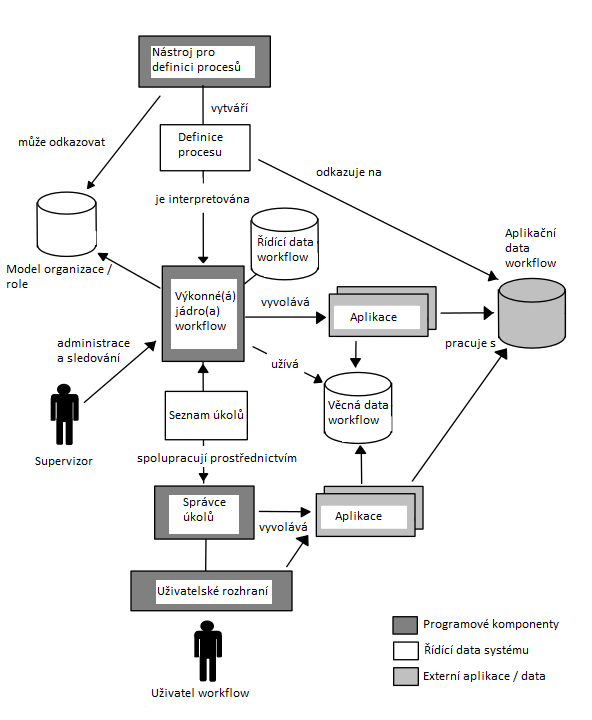
\includegraphics[width=340px]{images/obecny_model.png}
\caption{Obecný model workflow (převzato z \cite{wfmc})}
\end{figure}

Programové komponenty.

\begin{itemize}
\item Nástroj pro definici procesů (definition tool) umožňuje definovat procesy, přiřazovat role a stanovat pravidla.
\item Výkonné jádro workflow (workflow engine) řídí průběh workflow procesů, spouští nutné externí aplikace a udržuje statistiky o průběhu workflow.
\item Správce úkolů (worklist handler) má jako hlavní úkol zprostředkovávat komunikaci mezi jádrem workflow a jednotlivými uživateli.
\item Uživatelské rozhraní (user interface) zajišťuje komunikaci mezi správcem úkolů a uživatelem. Často tvoří jeden celek spolu se správcem úkolů.
\end{itemize}

Datové komponenty.

\begin{itemize}
\item Definice procesu (process definition) popisuje strukturu procesu.
\item Řídící data workflow (workflow control data) jsou interní data, které zpracovává jádro systému.
\item Aplikační data workflow (workflow application data) jsou specifická data aplikací.
\item Věcná data workflow (workflow relevant data) jsou data používaná jádrem k vyhodnocování dalších kroků.
\item Seznam úkolů (work list) představuje datovou strukturu, ve které jsou uloženy úkoly pro uživatele. Mohou být viditelné všechny najednou, nebo mu úkoly mohou být poskytovány postupně.
\item Model organizační struktury (organization/role model) popisuje organizační strukturu podniku. Pokud není definován, musí být úkoly přiřazovány pouze konktrétním uživatelům.
\end{itemize}

\subsection{Fáze workflow}
Obecně jsou rozlišovány dvě fáze workflow: fáze návrhu workflow a fáze průběhu workflow. \cite{workflow}

Fáze návrhu workflow v sobě zahrnuje funkce pro návrh a definici procesu, které jsou poskytovány analytickými a modelovacími nástroji. Ty umožňují převod procesu z reálného světa do normalizované podoby. Výsledkem je počítačově zpracovatelný popis procesu ve smyslu: kdo, kdy, co, s čím, za jakým účelem a jak má udělat.

Fáze průběhu workflow se dále dělí na funkce pro řízení běhu procesu, které zabezpečují interpretaci procesu, spouštění, provádění a kontrolu průběhu jednotlivých činností. Další část této fáze představuje interakce s uživateli a aplikačními nástroji. To například znamená předávání úkolů ke zpracování, vyžádání manuální činnosti, automatické spouštění jiných aplikací či předávání dat mezi aplikacemi.

Vše znárorněno na následujícím obrázku.

\begin{figure}[htp]
\centering
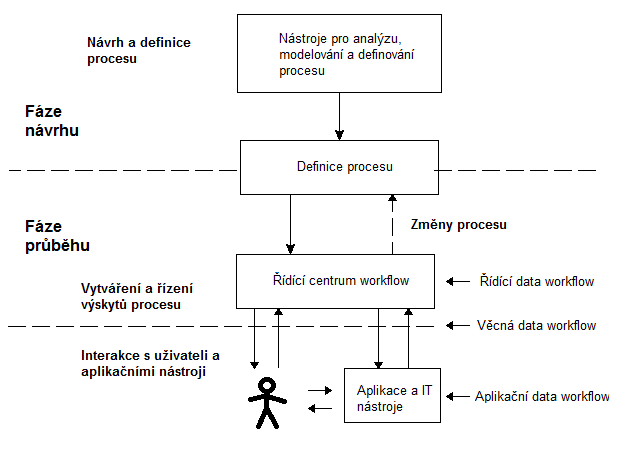
\includegraphics[width=340px]{images/faze_workflow.png}
\caption{Fáze workflow (převzato z \cite{wfmc})}
\end{figure}

\chapter{BPMN}
Buisiness Process Model And Notation (BPMN) je standard pro modelování podnikových procesů, jehož výstupem bývá grafické znázornění podnikových procesů v podobě procesních diagramů. \cite{bpmn} Jazyk BPMN také pomáhá sjednocovat významy základních pojmů používaných v této oblasti procesního řízení. 

Hlavním účelem BPMN je podporovat procesní řízení. Pro tuto funkci poskytuje notaci, která je jednoduchá, srozumitelná a intuitivní i pro netechnické pracovníky a zároveň dostatečná i pro vyjádření komplexních procesů. Přináší tedy standardizovaný zápis ve srozumitelné podobě pro všechny zainteresované osoby v organizacích.

Poslední verze BPMN 2.0 byla vydána v lednu 2011 a klade si za cíl být jedinou notací pro tvorbu modelů podnikových procesů. Proto mezi základními rysy jsou:
\begin{itemize}
\item snaha vytvořit jednotný konzistentní jazyk sjednocením definice podnikových procesů BPMN,
\item možnost vytvořit nezávislý nebo integrovaný model,
\item podpora a možnost výměny odlišných pohledů na procesní model tak, že je možno se v procesu zaměřit na slabá místa,
\item poskytnout xml schémata sloužící pro transformaci modelů.
\end{itemize}

\section{Základní notace}
Objekty jazyka BPMN jsou děleny do těchto základních kategorií. Tokové objekty, spojovací objekty, plavecké dráhy a artefakty. \cite{12}

\subsection{Tokové objekty}
Bývají označovány jako hlavní grafické prvky definující firemní procesy a dále se dělí.

\begin{itemize}
\item Události představují děje či události, ke kterým dochází v průběhu procesu.
\item Aktivity vyjadřují činnosti, které se odehrávají uvnitř procesu. Ty se dále dělí úlohy a podprocesy.
\item Brány jsou využívány pro zobrazení větvení a slučování toků a procesů, kdy je potřeba zohlednit různé podmínky. Dále jsou děleny na exkluzivní, inkluzivní a paralelní.
\end{itemize}

\begin{figure}[htp]
\centering

\includegraphics[width=210px]{images/tokove_objekty.png}
\caption{Tokové objekty}
\end{figure}


\subsection{Spojovací objekty}
Spojové objekty slouží ke spojování tokových objektů. Dělí se na sekvenční tok, tok zpráv a asociaci.

\begin{itemize}
\item Sekvenční tok znázorňuje posloupnost procesních toků v bazénu nebo podprocesu. Zdrojem a cílem je vždy nějaký tokový objekt. 
\item Tok zpráv označuje zprávy proudící přes hranice bazénů.
\item Asociace se používá pro připojení artefaktů nebo textu k tokovým objektům.
\end{itemize}

\begin{figure}[htp]
\centering
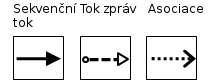
\includegraphics[width=210px]{images/spojovaci_objekty.png}
\caption{Spojovací objekty}
\end{figure}


\subsection{Plavecké dráhy}
Plavecké dráhy, někdy nazývané kontexty, slouží k organizování a kategorizaci činností. Rozlišují se typy: bazén a dráha.

\begin{itemize}
\item Bazén odděluje různé části popisované organizace.
\item Dráhy jsou součástí bazénu a používají se ke kategorizaci činností v rámci bazénu.
\end{itemize}

\begin{figure}[htp]
\centering
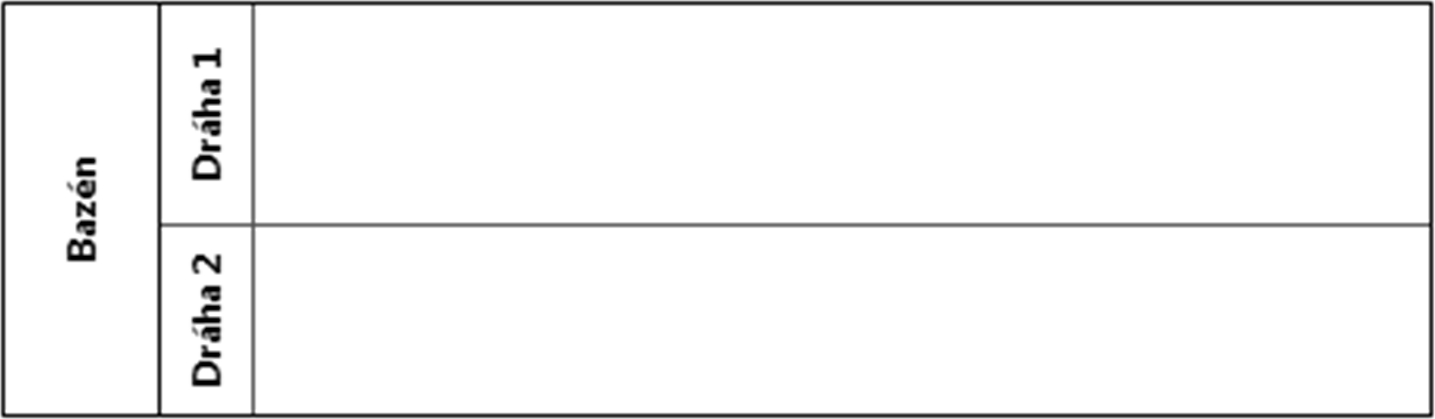
\includegraphics[width=340px]{images/bazen.png}
\caption{Bazén}
\end{figure}

\subsection{Artefakty}
Artefakty umožňují přidávat další informace do modelu a tím rozšiřují dostupné elementy v BPMN. Tím mohou zvyšovat informační hodnotu modelu. Existují tyto artefakty: datové objekty, skupiny a anotace.

\begin{itemize}
\item Datové objekty reprezentují nezbytná data pro vykonání dané činnosti.
\item Skupiny jsou využívány pro seskupení různých aktivit.
\item Anotace dodávají modelu srozumitelnost a přehlednost.
\end{itemize}

\begin{figure}[htp]
\centering

\includegraphics[width=340px,height=70px]{images/artefakty.png}
\caption{Artefakty}
\end{figure}

\chapter{Volba workflow engine pro Liferay}


Portál Liferay implementuje služby pro workflow tak, že může být využito skrze celý portál a může být využito jak pro publikování webového obsahu, schválování článku blogu, pro práci s dokumenty a v dalších oblastech.

Liferay je v základní edici dodáván s workflow systémem Kaleo, který je jednoduchý a snadnou použitelný a plně dostačuje k základnímu použití pro práci s webovým obsahem nebo pro práci s dokumenty. Pro složitější a komplexenější workflow umžňuje Liferay využít i jiné a rozsáhlejší workflow systému, jako například Activiti nebo JBoss's jBPM. Vždy ale musí být použit na portálu právě jeden workflow systém, proto je nutné před nasazením zvolit ten nejvhodnější.

\begin{itemize}
\item Activiti. Projekt Activiti vznikl v roce 2010 a jeho cílem bylo vytvořit svobodné výkonné jádro workflow, které bude podporovat specifikaci BPMN 2.0. Toto výkonné jádro může být využíváno samostatně nebo může být vloženo do jiného systému.
\item JBoss's jBPM.
\item Kaleo.
\end{itemize}

\subsection{Activiti}


\chapter{Analýza a návrh grafického designeru}





\chapter{Závěr}

%\printindex

\begin{thebibliography}{0}

\bibitem{gala}
GÁLA, L. et al. \textit{Podniková informatika}. 1. vyd. Praha: Grada Publishing, 2006. 

\bibitem{jsr-286}
\textit{JavaTM Portlet Specification}, The Java Community Process, dostupný na \url{http://www.jcp.org/en/jsr/detail?id=286} [cit. 2014-03-27].

\bibitem{cech}
ČECH, P. \textit {Přinos podnikových portálů pro management znalostí}, in Internet a konkurenceschopnost, Zlín, 2004.

\bibitem{enterprise-portal}
\textit{Enterprise portal}, Wikipedia, dostupný na \url{http://en.wikipedia.org/wiki/Enterprise_portal} [cit. 2014-03-27].

\bibitem{developer-guide}
\textit{Liferay Portal 6.2 Developer's Guide}, Liferay Inc., dostupný na \url{http://www.liferay.com/documentation/liferay-portal/6.2/development} [cit. 2014-04-02].

\bibitem{liferay-features}
\textit{Portal Features}, Liferay Inc., dostupný na \url{http://www.liferay.com/products/liferay-portal/features/portal} [cit. 2014-04-02].

\bibitem{portlets-in-action}
SARIN, Ashish. \textit{Portlets in action}, Shelter Island, NY: Manning, 2011.

\bibitem{wfmc}
\textit{Terminology \& Glossary}, Workflow Management Coalition, dostupný na \url{http://www.wfmc.org/standards/docs/TC-1011_term_glossary_v3.pdf} [cit. 2014-04-14].

\bibitem{workflow}
CARDA, A., KUNSTOVÁ, R. \textit {Workflow : Nástroj manažera pro řízení podnikových procesů}. 2. vyd. Praha: Grada Publishing, 2003.

\cite{bpmn}
\textit{Business Process Model and Notation (BPMN)}, Object Management Group, Inc., dostupný na \url{http://www.omg.org/spec/BPMN/2.0/} [cit. 2014-04-23]


\end{thebibliography}


\newpage
\appendix
\chapter{Položky seznamu}
asdfsadf


\end{document}